%%%%%%%%%%%%%%%%%%%%%%%%%%%%%%%%%%%%%%%%%
% Thin Sectioned Essay
% LaTeX Template
% Version 1.0 (3/8/13)
%
% This template has been downloaded from:
% http://www.LaTeXTemplates.com
%
% Original Author:
% Nicolas Diaz (nsdiaz@uc.cl) with extensive modifications by:
% Vel (vel@latextemplates.com)
%
% License:
% CC BY-NC-SA 3.0 (http://creativecommons.org/licenses/by-nc-sa/3.0/)
%
%%%%%%%%%%%%%%%%%%%%%%%%%%%%%%%%%%%%%%%%%

%----------------------------------------------------------------------------------------
%	PACKAGES AND OTHER DOCUMENT CONFIGURATIONS
%----------------------------------------------------------------------------------------

\documentclass[a4paper, 11pt]{article} % Font size (can be 10pt, 11pt or 12pt) and paper size (remove a4paper for US letter paper)

\usepackage[usenames, dvipsnames]{color}
\usepackage[protrusion=true,expansion=true]{microtype} % Better typography
\usepackage{subfigure}
\usepackage{graphicx} % Required for including pictures
\usepackage{wrapfig} % Allows in-line images

\usepackage{mathpazo} % Use the Palatino font
\usepackage[T1]{fontenc} % Required for accented characters



\usepackage{url} % para que aparezcan las url de las paginas web. En el archivo bib hay que poner howpublished = "\url{URL del recurso}"
\usepackage[nottoc,numbib]{tocbibind} % para que la bibliografia aparezca en la tabla de contenidos (toc) numerada adecuadamente (numbib)
\usepackage{listings} % para introducir codigo bonito
\usepackage{textcomp} % hace falta para poner apostrofe ' -.-''''''''
\usepackage{gensymb} % para que \degree introduzca el simbolo 
\usepackage[hidelinks]{hyperref} %clickable index
\hypersetup{
    colorlinks=false, %set true if you want colored links
    linktoc=all,     %set to all if you want both sections and subsections linked
%    linkcolor=blue,  %choose some color if you want links to stand out
}

\usepackage[export]{adjustbox} % Para generar bordes negros en las figuras

%\definecolor{black}{rgb}{0,0,0} % Example color definition, the color can be used with the \color{name} command
%\definecolor{red}{rgb}{1,0,0} % Example color definition, the color can be used with the \color{name} command

\linespread{1.05} % Change line spacing here, Palatino benefits from a slight increase by default

\makeatletter
\renewcommand\@biblabel[1]{\textbf{#1.}} % Change the square brackets for each bibliography item from '[1]' to '1.'
\renewcommand{\@listI}{\itemsep=0pt} % Reduce the space between items in the itemize and enumerate environments and the bibliography

\renewcommand{\maketitle}{ % Customize the title - do not edit title and author name here, see the TITLE block below
\begin{flushright} % Right align
{\LARGE\@title} % Increase the font size of the title

\vspace{50pt} % Some vertical space between the title and author name

{\large\@author} % Author name
\\\@date % Date

\vspace{40pt} % Some vertical space between the author block and abstract
\end{flushright}
}

\usepackage[english]{babel}
\usepackage{framed}
\usepackage{listings}             % Include the listings-package

% Default fixed font does not support bold face
\DeclareFixedFont{\ttb}{T1}{txtt}{bx}{n}{12} % for bold
\DeclareFixedFont{\ttm}{T1}{txtt}{m}{n}{12}  % for normal

% Custom colors
\usepackage{color}
\definecolor{deepblue}{rgb}{0,0,0.5}
\definecolor{deepred}{rgb}{0.6,0,0}
\definecolor{deepgreen}{rgb}{0,0.5,0}

\usepackage{listings}

% Python style for highlighting
\newcommand\pythonstyle{\lstset{
language=Python,
basicstyle=\ttm,
otherkeywords={self},             % Add keywords here
keywordstyle=\ttb\color{deepblue},
emph={MyClass,__init__},          % Custom highlighting
emphstyle=\ttb\color{deepred},    % Custom highlighting style
stringstyle=\color{deepgreen},
frame=tb,                         % Any extra options here
showstringspaces=false            % 
}}


% Python environment
\lstnewenvironment{python}[1][]
{
\pythonstyle
\lstset{#1}
}
{}


\setlength{\parindent}{2em}
\setlength{\parskip}{1em}


%----------------------------------------------------------------------------------------
%	TITLE
%----------------------------------------------------------------------------------------

\title{\textbf{Structural Bioinformatics Final Exam}\\  % Title
\vspace{10pt}Protein Part} % Subtitle

\author{\textsc{Antonio Ortega Jim\'enez} % Author
\\{\textit{University of Copenhagen}}} % Institution

\date{\today} % Date

%----------------------------------------------------------------------------------------

\begin{document}

\maketitle % Print the title section
\thispagestyle{empty}

\vspace{-3.7cm}
\begin{figure}[!h]

\includegraphics[scale=0.35]{figures/ku_logo}
\end{figure}

\vspace{30pt}

\begin{center}
\Huge{\textbf{RMSD analysis on identical n-mers in the top100H database}}
\end{center}

\begin{figure}[!h]
\begin{center}
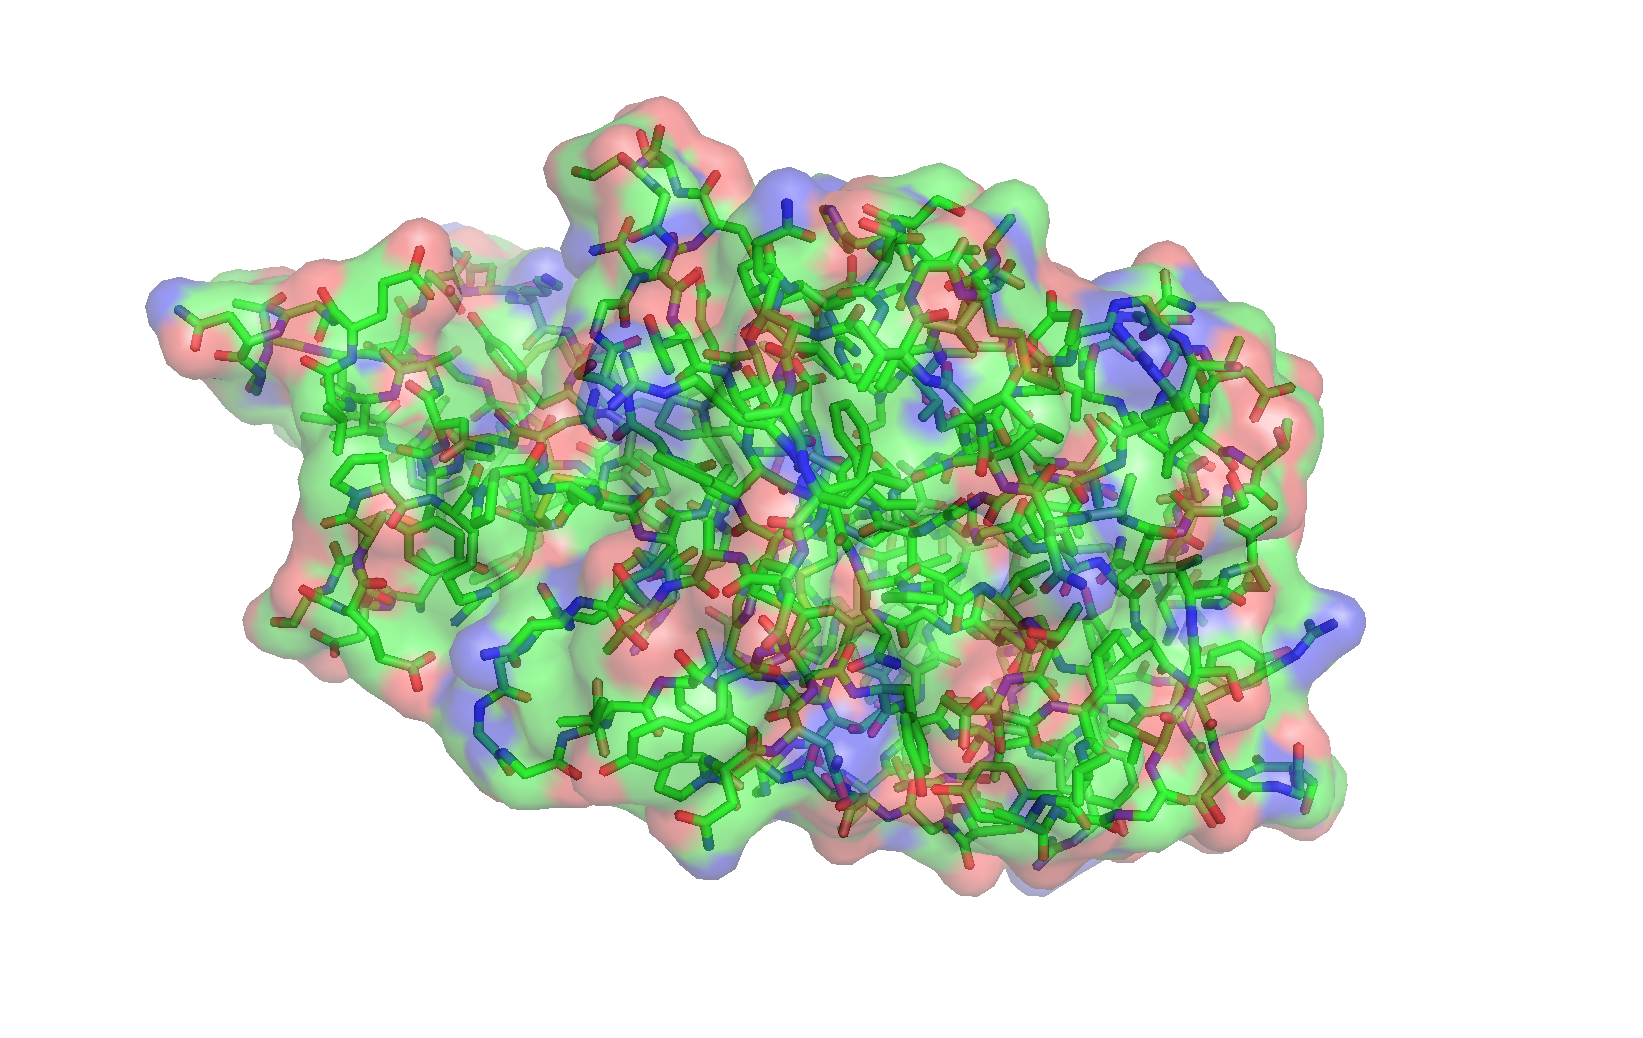
\includegraphics[scale=0.25]{../plots/cover}% tight frame
\end{center}
\end{figure}




\newpage
%----------------------------------------------------------------------------------------
%	INDICE
%----------------------------------------------------------------------------------------

\setcounter{figure}{0}
\renewcommand\thefigure{\arabic{figure}}
%\renewcommand{\figurename}{\textbf{Figura}}
%
\setcounter{table}{0}
\renewcommand\thetable{\arabic{table}}
%\renewcommand{\tablename}{\textbf{Tabla}}

\thispagestyle{empty}
\tableofcontents
\thispagestyle{empty}

\newpage



%----------------------------------------------------------------------------------------
%	ESSAY BODY
%----------------------------------------------------------------------------------------

\setcounter{page}{1}
\section{Introduction}

The study of protein structure is a hot topic on several fields like medicine and the biotech industry. For that matter, Bioinformatics methods that predict and analyze structure information are constantly being developed by the scientific community. Moreover, since research groups all around the world publish their results on open databases this methods can be easily be applied to real data. One of such databases is the Protein Data Bank, maintained by an international consortium. In other words, bioinformaticians have both open data and free software to try out new ideas.

%ref PDB

Do we expect structure similarity in identical sequences of n residues? Aminoacidic sequence has a great impact on secondary structure, up to making some conformations highly unlikely. This is due to the particular spatial properties and constraints each different kind of aminoacid shows. Thus, we should expect a general trend toward similarity in sequence pairs of short lengths, for short sequences acquire very little degree of \textquotesingle conformational\textquotesingle freedom.

On the other hand, structural similarity between a pair of structures can be modelled using the Root Mean Square Deviation (RMSD) statistic. While a small value of this parameter tells us that the pair of structures has high similarity, a big value indicates no similarity at all.
%ref RMSD

In this report, a simple \textit{in silico} analysis of protein structure data was run to try to give an answer to this question. The Biopython module, contained in the Python programming language, together with the statistical language R, were used for extracting all possible n-mers in a protein database and computing their RMSD values. The default length of the n-mers was set to 5, but data for n from 3 to 20 was generated.

%ref Biopython

\section{Materials and methods}


\subsection{Structure and sequence parse, and generation of n-mers}


\begin{quote}
\textit{Classroom data are like teddy bears and real data are like a 
grizzley bear with salmon blood dripping out its mouth.}

\hfill Jenny Bryan
\end{quote}

Real data come messy and in ways that make very hard to learn knowledge from it. The dataset provided in this report fitted one of those grizzley bears, for the reason explained in \textit{Rebuild of the top100H}.
 
Structural (spatial) information was parsed from the database by making use of the \texttt{PDBParser.get\_structure()} method, whereas sequence data was parsed using the \texttt{SeqIO.parse()}  method. Both of these functions are available in the Biopython package. Chain breaks, consisting of residues whose spatial information is either missing, or irrelevant (due to their disordered nature), were handled with several user defined functions. In a nutshell, this chain breaks were represented in the sequence set by replacing the letter of the affected aminoacids with X.

Fragments were generated with Python list\textquotesingle s comprehension:

\begin{verbatim}
[(seq[i:i + n], i) for i in range(0, len(seq) - n) \
if not "X" in seq[i:i + n]]
\end{verbatim}

This way, subsequences of length \textit{n} that do not contain X are stored in a list. This list represents all n-mers that can be extracted from sequence \textit{seq}.

Information relating to the n-mer sequence, position and geometrical coordinates was stored in a customized data type called \texttt{Fragment}:


\lstset{language=Python}          % Set your language (you can change the language for each code-block optionally)

\begin{python}
class Fragment(object):

    def __init__(self, seq, start, seq_id, \
    chain_id, X, atoms):
        self.seq = seq           # aminoacidic seq
        self.start = start       # start pos
        self.seq_id = seq_id     # pdb id of the protein
        self.chain_id = chain_id # chain id
        self.X = X               # coordinates matrix
        self.atoms = atoms
\end{python}





\subsection{Rebuild of the top100H}

The top100H database consists of a collection of a 100 files that represent a 100 different protein structures. It is available in this link:

\color{blue}
\href{http://kinemage.biochem.duke.edu/databases/top100.php}{http://kinemage.biochem.duke.edu/databases/top100.php}
\color{black}

A first usage of these files revealed several issues related to the out of date syntax that was employed in their creation. For that reason, the database was rebuilt using modern day files.
These new pdb files were downloaded using the \texttt{pdbList.retrieve\_pdb\_file()} method, available in Biopython. Entry ids were parsed from the ones in the original database. The scripts used to complete this are available at

\texttt{\href{https://github.com/antortjim/rmsd\_nmers/tree/master/database}{https://github.com/antortjim/rmsd\_nmers/tree/master/database}}.


\subsection{Pairwise computation of RMSD}

The computation of RMSD receives two matrices of dimensions described as below:

\begin{itemize}

\item Each column stores a coordinate vector that represents the position of a spatial entity. In this report, only C$\alpha$ atoms were used.

\item Each row stores one of the 3 dimensions in space.
\end{itemize}

Thus, in this report, n x 3 matrices were used, where every row represents the $C\alpha$ atom in each residue of the n-mer.

A structurally relevant RMSD has to be computed on two matrices X and Y that have been centered and rotated so that the RMSD is minimized. This requirement is fulfilled by means of a mathematical method called Singular Value Decomposition (SVD). This algorithm computes the rotational matrix required by Y to minimise RMSD. Together with a centering method, the RMSD can be brought to its minimum.

These are the key aspects of this combined SVD + RMSD calculation algorithm:

\begin{itemize}

\item Matrices are centered in the coordinates origin by substracting the center matrix (1 x 3) to all rows in the coordinates matrices. The center of the new matrices will now be 0, 0, 0.

\item Compute the correlation matrix R between X and Y (XT\textsuperscript{t}).

\item Perform SVD on this matrix and return 3 matrices V, S, and W\textsuperscript{t}.

\item The minimum RMSD can now be computed using the following formula.

$$RMSD = \sqrt { \frac { 1 }{ n }  ( E_0 - 2(\sigma_1 + \sigma_2 + \sigma_3 )}$$

where

$$E_0 = \sum _{ i=0 }^{ n-1 }(|x_i|^{2} + |y_i|^{2})$$

and the $\sigma$ summation is the sum of the S matrix.

\end{itemize}

This whole computation was achieved by making use of user defined functions and the svd implementation available at the Python module numpy (\texttt{numpy.linalg.svd()}).

User defined functions may be found in this link

\begin{center}
\texttt{\href{https://github.com/antortjim/rmsd\_nmers/blob/master/user\_defined.py}{https://github.com/antortjim/rmsd\_nmers/blob/master/user\_defined.py}}
\end{center}

\subsection{Visualization of data}

Interpretation and visualization of the data were performed in R using the ggplot2, data.table, dplyr, cowplot and Shiny packages. Briefly, the data generated with the Python scripts was loaded with R\textquotesingle s \texttt{read.csv()}. The random and sequence pairs data were merged using \texttt{dplyr::full\_join()}. Duplicates were detected using data.table methods and finally, graphics were generated using ggplot2. The interactive website was built with Shiny.

\section{Results}


\subsection{RMSD values distribution for 5-mers}

As previously explained, the RMSD values obtained in real sequence pairs was expected to be significantly different from those obtained in random matches (with no sequence similarity). As shown in figure \ref{fig:hist}, this was the case. 

\begin{figure}[!h]
\begin{framed}
\centering
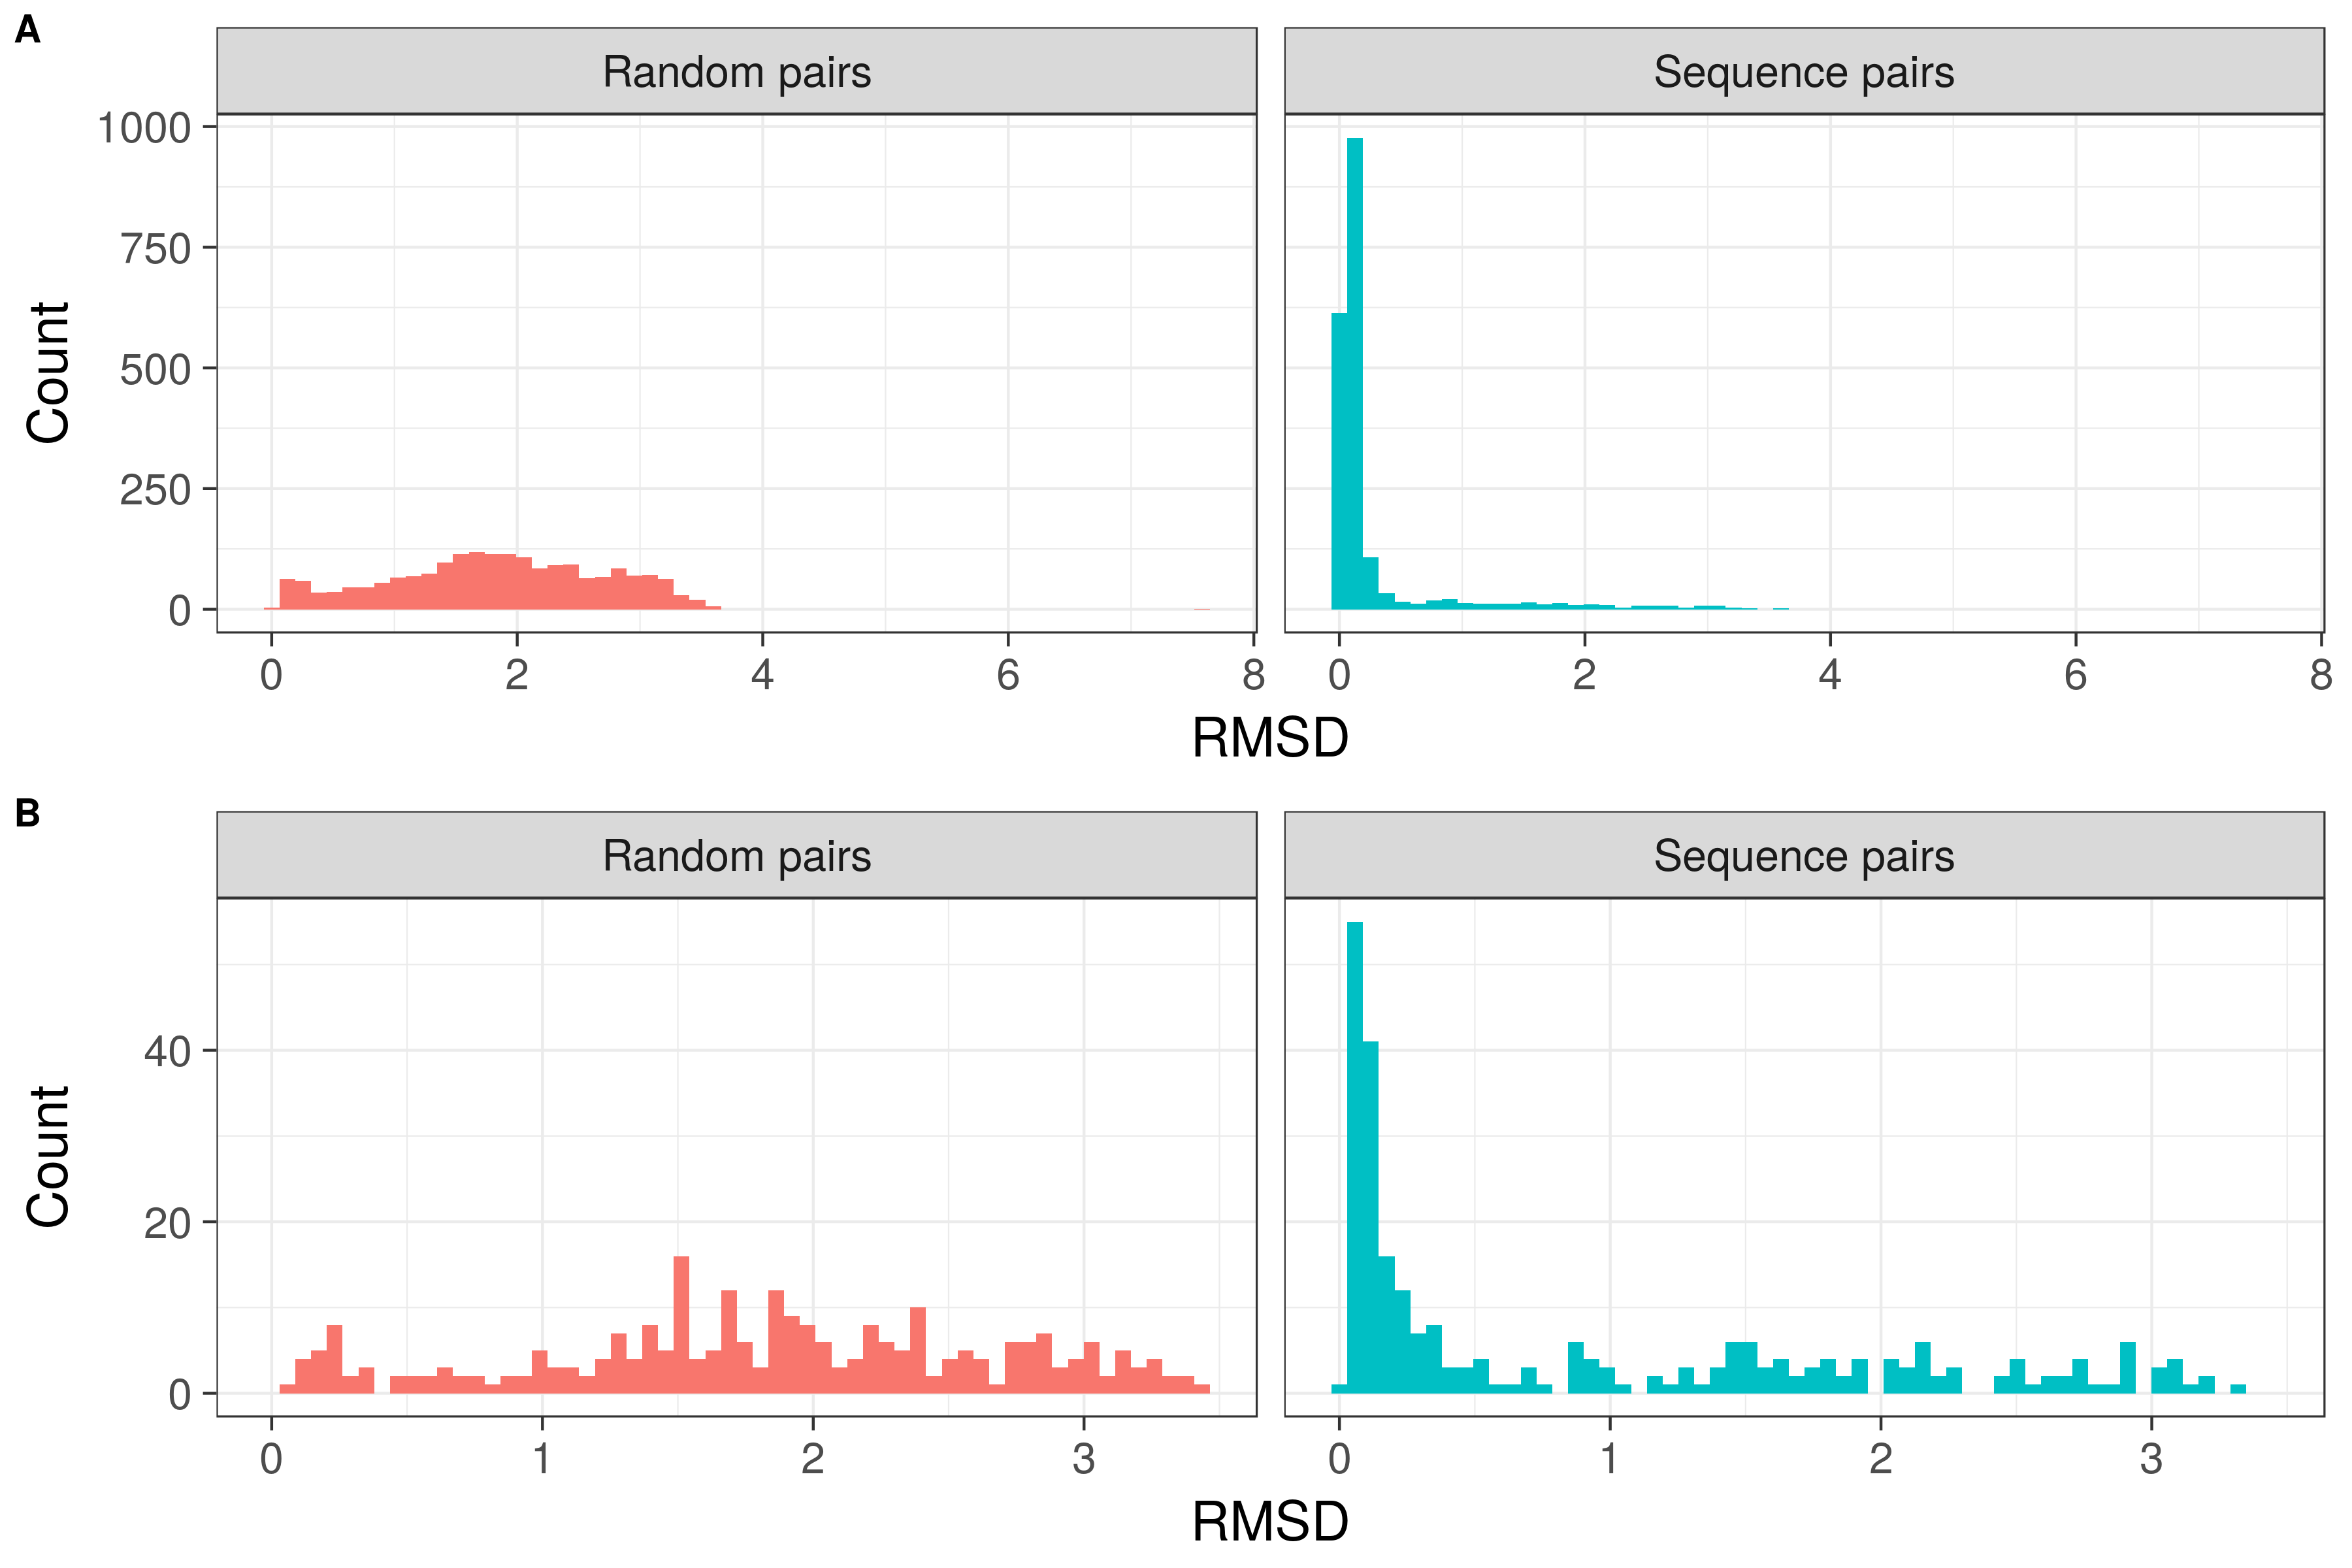
\includegraphics[width = \textwidth]{../plots/histogram.png}
\caption{\textbf{5-mers RSMD distribution histograms}. \textbf{A} If all intraprotein matches and those occuring in structure-sharing proteins are included, an exaggerated count is obtained for low RMSD values. \textbf{B} If matches from the same protein are discarded, and only the first of those in structure-sharing proteins are taken into account, a more sensible distribution is obtanined. In both cases, a clear trend toward low values is observed in sequence pairs, whereas no particular trend is observed in sequences paired at random. No peak, besides the one at very low RMSD values, was observed.}
\label{fig:hist}
\end{framed}
\end{figure}

A total of 266 fragments fell in the latter category. The median RMSD value for the random pairs was 1.86, and only 0.33 in the sequence pairs.

\subsection{Proteins under PDB entries 4ptp and 1mct share a domain}

Notably, a huge amount of sequence pairs were found between the same pair of proteins. It was specially true for the pair of proteins with ids 4ptp and 1mct. This pair exhibited 81 5-mer matches. 

The existence of this and other matching-prone pairs was easily spotted in the preliminar histogram of the RMSD values (fig \ref{fig:hist} A), which showed a extremely high count at very low RMSD values. This is due to the fact that matching-prone pairs most likely share domains, and consequently return a high count of 5-mers with low RMSD values.

The 4ptp and 1mct pair was further explored. First, in order to check the presence of a shared domain, the Pfam database 
%ref Pfam
was queried. Indeed, both proteins share a Trypsin domain. Secondly, this domain was visualized using the Pymol suite (fig. \ref{fig:perfect_match}). The alignment of both structures confirms that they share a domain.

\begin{figure}[!h]
\begin{center}
    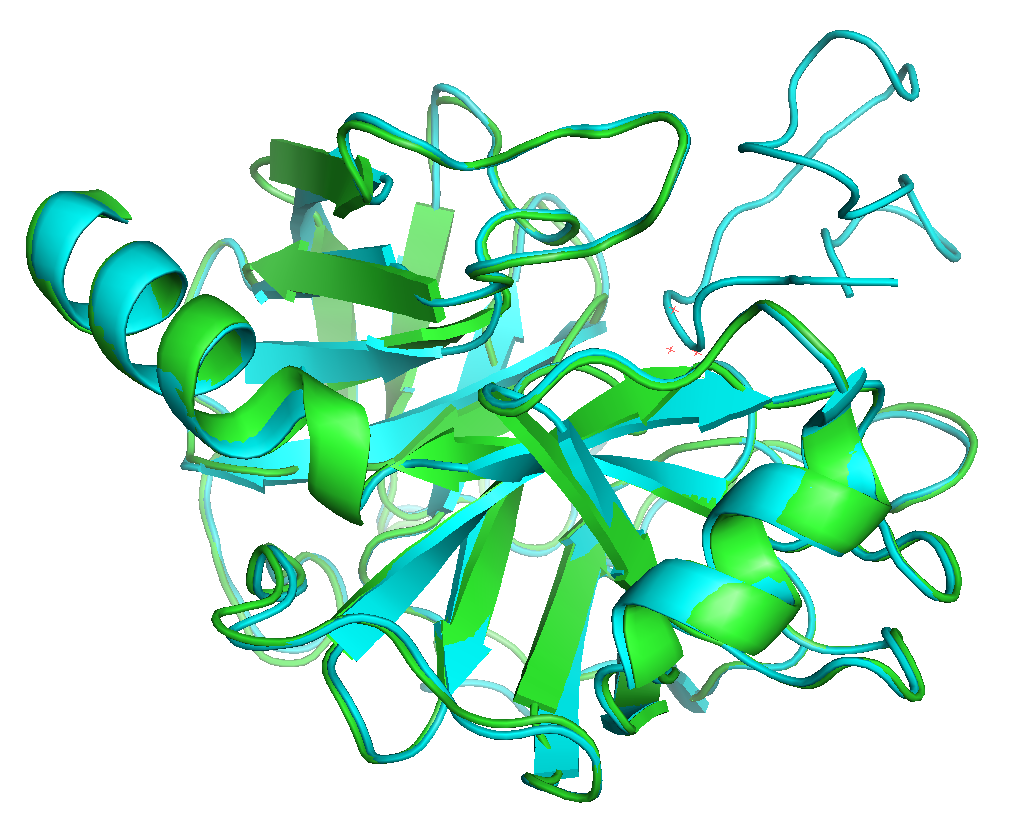
\includegraphics[width = 0.5\textwidth]{../plots/perfect_match_white.png}
  \end{center}
  \label{fig:perfect_match}
  \caption{4ptp and 1mct are highly similar.}
\end{figure}

\subsection{Sequence pairs with high RMSD values adopt opposite conformations}

As well as sequence pairs with low RMSD values, many with higher RMSD values were detected. Let us visualize, the pair with sequence ALTAA. This pair is found in two proteins:

\begin{itemize}

\item Chain A and residue 64 in protein 1aru.

\item Chain A and residue 231 in protein 1nif

\end{itemize} 

This pair exhibited a RMSD value of 3.13, one of the highest for a sequence pair. A visualization of their structure (fig \ref{fig:high_rmsd}) reveals the reason behind it: In 1aru, this sequence adopts an $\alpha$ fold, whereas in 1nif, it adopts $\beta$ conformation.


\begin{figure}[!h]
\begin{center}
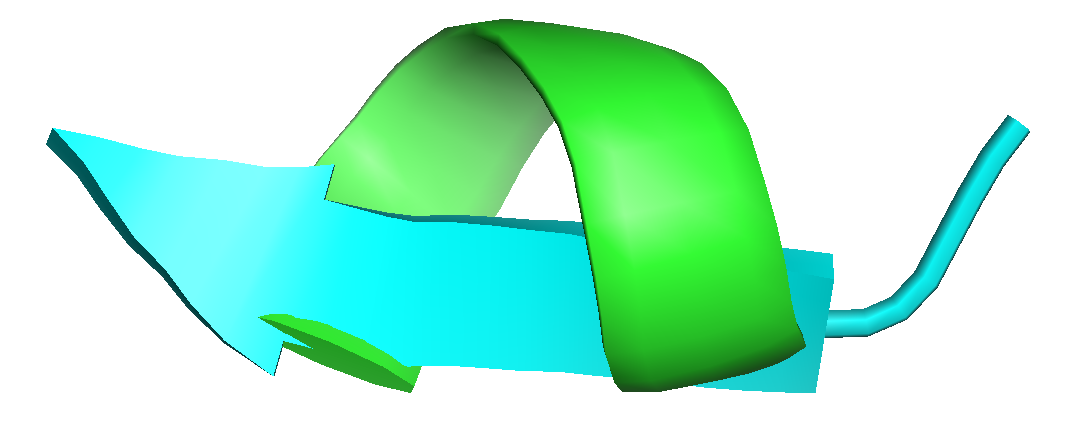
\includegraphics[width = 0.5\textwidth]{../plots/high_rmsd.png}
\end{center}

\label{fig:high_rmsd}
\caption{Even though they share aminoacidic sequence, this pair of 5-mers adopts a totally different fold that leads to an RMSD value of 3.13.}
\end{figure}

\subsection{Increasing the size of the n-mers promotes the divergence of the sequence pairs distribution}

As a proof of concept, the whole analysis was repeated for 10-mers, that is, for pairs of aminoacidic sequences of length 7. Longer sequences increase the degrees of structural conformation freddom. This should spread out the random pairs distribution around larger RMSD values (fig \ref{fig:7mers}). At the same time, only sequence pairs with low RMSD values will remain, for long sequence sharing is found only in domain families, which of course have very similar structures.

\begin{figure}
\begin{center}
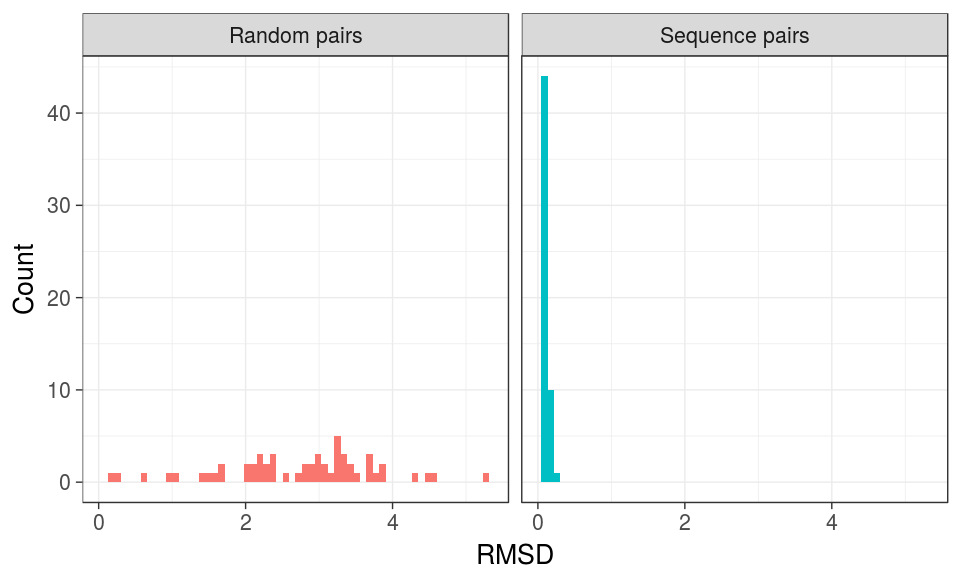
\includegraphics[width = 0.8\textwidth]{../plots/7mers.png}
\caption{The 7-mers random pairs distribution spreads around a larger interval of RMSD values. The sequence pairs distribution moves toward lower values, while the random pairs become more spread out and move toward larger values. The number of n-mers decreases because matches are less probable.}
\label{fig:7mers}
\end{center}
\end{figure}


\subsection{Interactive visualization of RMSD distributions}

A visualization of the random and sequence pair distributions obtained for n-mers of lengths ranging from 3 to 20 can be obtained in this link:

\color{blue}
\texttt{\href{https://antortjim.shinyapps.io/sb\_exam/}{https://antortjim.shinyapps.io/sb\_exam/}}
\color{black}

\section{Conclusions}

This report has delved into the relationship between structure and sequence. Root Square Mean Deviation has proved to be an efficient statistic to measure the difference between 2 sets of coordinates. RMSD distributions show that short sequence sharing fragments are prone to share their structure as well. This trend is accentuaded as the length of the fragments is extended. This is opposite to what can be observed in random pairs, that show no trend to particular low RMSD values. Moreover, as the length of the fragments grows the RMSD distribution skews to larger values. This is explained by the the exponential increase in the number of degrees of freedom, that make structures diverge to a greater range of possible conformations.

Quite a lot of the observed matches came from only a few pair of proteins, and they happeneded to at least partially share their structure This shows that once a match is found between a pair of proteins, the pair becomes more likely to eventually yield more matches, due precisely to the fact that they indeed share structure at some extent. Protein comparison methods could take advantage of this property implementing n-mer seeds that heuristically accelerate algorithms.

The number of detected n-mers was extremely dependent of their length, so that only 74 6-mers are found. This suggests that further analysis with a significant amount of fragments will require larger datasets, with thousands of protein entries. For example, a filtered subset of the PDB could be valid for such an analysis.

Finally, bioinformatics methods for data analysis have proved to be very useful and effective in the performance of complex tasks. Still, Biopython does not provide a secondary structure parsing module, and DSSP, the recommended alternative, is not well integrated with the rest of the module. There is work to be done. 

%\nocite{hadley2009}
%\nocite{sonrisa}

%%----------------------------------------------------------------------------------------
%%	BIBLIOGRAPHY
%%----------------------------------------------------------------------------------------
%
\bibliographystyle{unsrt}
%\bibliography{bibliografia}
%%----------------------------------------------------------------------------------------

\end{document}
